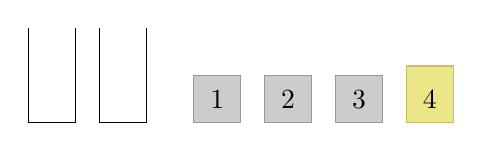
\begin{tikzpicture}[scale = 0.6]

  %%%%%%%%%%%Draw the first bin%%%%%%%%%%%
  \draw (0,0) -- (0,-2);
  \draw (0,-2) -- (1,-2);
  \draw (1,-2) -- (1,0);

  %%%%%%%%%%%Draw the second bin%%%%%%%%%%
  \draw (1.5,0) -- (1.5,-2);
  \draw (1.5,-2) -- (2.5,-2);
  \draw (2.5,-2) -- (2.5,0);

  %%%%%%%%%%%Draw 4 items%%%%%%%%%%%%%%%%%
  \filldraw[fill=gray!40,draw=gray!80] (3.5,-2) rectangle (4.5,-1);
  \draw (4,-1.5) node {1};
  \filldraw[fill=gray!40,draw=gray!80] (5,-2) rectangle (6,-1);
  \draw (5.5,-1.5) node {2};
  \filldraw[fill=gray!40,draw=gray!80] (6.5,-2) rectangle (7.5,-1);
  \draw (7,-1.5) node {3};
  \filldraw[fill=gray!30!yellow!60,draw=yellow!50!gray] (8,-2) rectangle (9,-0.8);
  \draw (8.5,-1.5) node {4};
\end{tikzpicture}
  %%%%%%%%%%%%%%%%Optimum integer packing%%%%%%%%%%%%%%
  \pause
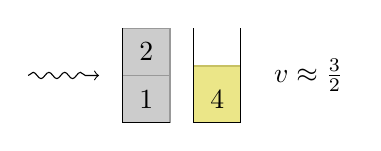
\begin{tikzpicture}[scale = 0.6]
  %right arrow
  \draw [->,decorate, decoration={snake,amplitude=.4mm,segment length=2mm,post length=1mm}]
  (10,-1) -- (11.5,-1);

  \filldraw[fill=gray!40,draw=gray!80] (12,-2) rectangle (13,-1);
  \draw (12.5,-1.5) node {1};
  \filldraw[fill=gray!40,draw=gray!80] (12,-1) rectangle (13,0);
  \draw (12.5,-0.5) node {2};
  \filldraw[fill=gray!30!yellow!60,draw=yellow!50!gray] (13.5,-2) rectangle (14.5,-0.8);
  \draw (14,-1.5) node {4};

  \draw (12,0) -- (12,-2);
  \draw (12,-2) -- (13,-2);
  \draw (13,-2) -- (13,-2);

  \draw (13.5,0) -- (13.5,-2);
  \draw (13.5,-2) -- (14.5,-2);
  \draw (14.5,-2) -- (14.5,0);

  \draw (15,-1) node[right] {$v\approx \frac{3}{2}$};
\end{tikzpicture} 